\chapter{Grundlagen}
\label{cha:grundlagen}
Um die Nachvollziehbarkeit der folgenden Inhalte zu gewährleisten, bereitet dieses Kapitel zunächst die Grundlagen auf. Es stellt vergleichbare Technologien vor und diskutiert verschiedene Ansätze zum Tracking von Nutzerverhalten. Darüber hinaus erläutert es zwei weitere Patterns, die speziell in der UI-Entwicklung zum Einsatz kommen und für das betrachtete System von Bedeutung sind.

\section{Vergleichbare Anwendungen}
\label{sec:similar_applications}
Speziell im Webbereich stehen bereits einige Frameworks und Systeme zur Verfügung, die es einfach und effizient machen, Nutzerverhalten aufzuzeichnen. Web und native Technologien unterscheiden sich zwar in vielen Aspekten, dennoch lassen sich einige Konzepte übertragen. Zwei der größten Vertreter von OpenTelemetry und Google sind daher in diesem Abschnitt beschrieben. Zu erwähnen ist, dass der Fokus auf der Datenermittlung der Systeme liegt, da die Analyse unabhängig von der Technologie anwendbar ist und die Problemstellung auf der Datenerfassung liegt.

\subsection{Google Analytics}
\label{subsec:google_analytics}

Google Analytics ist ein Tool, das auf der Technologie der Urchin Software Corporation basiert, die 2005 von Google übernommen wurde \cite{google2005urchin}. Ziel von Google Analytics ist es, Website-Betreibern mithilfe gesammelter Daten einen Überblick über die Nutzung ihrer Seiten zu verschaffen. Die gewonnenen Informationen sollen Unternehmen dabei unterstützen, ihre Marketingmaßnahmen gezielt zu steuern und deren Wirkung zu steigern.

\subsubsection{Technologie Überblick}
Die von Google bereitgestellte Abbildung \ref{fig:googel_analytics_architecture} zeigt die Architektur von Google Analytics und gibt einen Überblick über die verschiedenen Nutzungsmöglichkeiten. Wie zu Beginn des Abschnitts \ref{sec:similar_applications} beschrieben, ist Google einer der Vertreter, die eine flexible Schnittstelle zur Bereitstellung der Daten anbieten. In der Abbildung \ref{fig:googel_analytics_architecture} werden daher beispielhaft die Nutzungsmöglichkeiten über Web-Client, Server und Mobile aufgezeigt.
Wesentlich ist jedoch, dass die Daten in der im "Measurement Protocol" \cite{google_developers_sending_events} beschriebenen Form übermittelt werden. Die Auswertung der gesammelten Daten über die dargestellte Google Analytics-Benutzeroberfläche wird in dieser Arbeit nicht behandelt. Dennoch stellt Google für die drei genannten Plattformen Frameworks bereit, die eine automatische und vereinfachte Datensammlung ermöglichen und für diese Arbeit von Relevanz sind.

\begin{figure}[h]
\centering
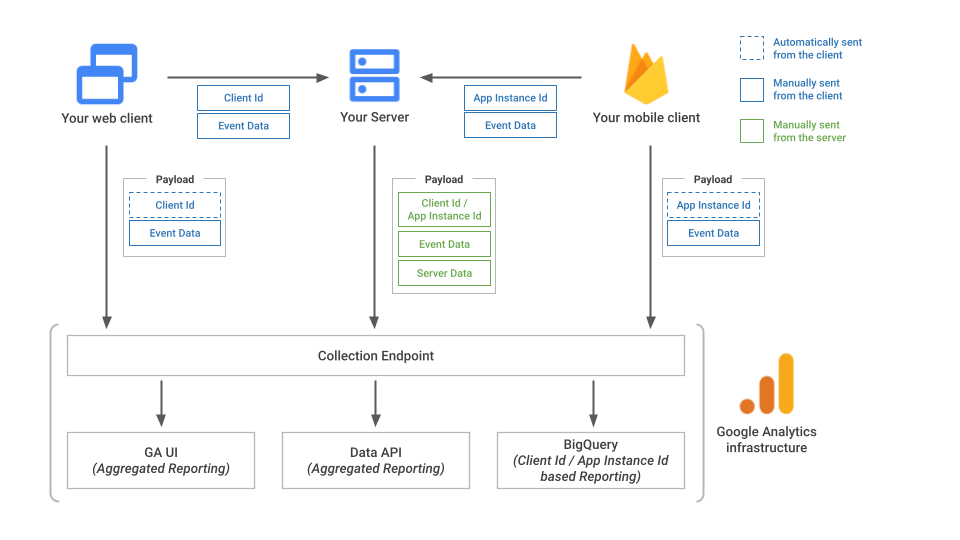
\includegraphics[width=0.95\textwidth]{2_Architektur_Google_Analytics}
\caption{Architektur Google Analytics. Quelle \cite{google_developers_sending_events}}
\label{fig:googel_analytics_architecture}
\end{figure}

\subsubsection{Technologie für Webseiten}
Einer der in Abbildung \ref{fig:googel_analytics_architecture} dargestellten Datenquellen ist eine Webseite. 
Für deren Integration stellt Google JavaScript-Code bereit, der lediglich in die Webseite eingefügt werden muss. 
Sobald der Client dieses Skript ausführt, lädt es automatisch weitere Skripte von Google nach, welche die Ausführung vordefinierter und benutzerdefinierter Kommandos ermöglichen. 
Über diese Kommandos werden die Daten gemäß dem \textit{Measurement Protocol} \cite{google_developers_sending_events} an Google übermittelt. 
Dadurch ergibt sich folgende Datenhierarchie:

\begin{enumerate}
    \item \textbf{Hit}: Ein einzelner Datensatz, beispielsweise ein Ereignis wie ein Button-Klick.
    \item \textbf{Session}: Eine Sammlung mehrerer Ereignisse, die während einer Sitzung auftreten.
    \item \textbf{Property}: Fasst alle Hits zusammen, die mit derselben Property-ID gekennzeichnet sind (z.\,B. alle Daten einer Webseite).
    \item \textbf{View}: Repräsentiert eine bestimmte Ansicht oder einen gefilterten Ausschnitt der Daten einer Property.
\end{enumerate}

Die Daten können auf verschiedene Weise übermittelt werden. Eine dieser Varianten ist die Ausführung des in Programm \ref{prog:send_command} dargestellten JavaScript-Codes. Wie zu erkennen ist, werden die Daten in unterschiedliche Kategorien unterteilt, um spätere Filterungen und Abfragen zu erleichtern.

\begin{program}[H]
\begin{JsCode}
ga('send', 'social', 'network', 'action', 'target');
\end{JsCode}
\caption{Sende-Kommando in Google Analytics}
\label{prog:send_command}
\end{program}

Um den Quellcode übersichtlich zu halten und das Tracking flexibel zu gestalten, bietet Google zusätzlich den sogenannten \textit{Tag Manager} an. 
Tags stellen hierbei Code- oder HTML-Elemente dar, die je nach definierten Bedingungen (Triggern) automatisch in die Webseite eingefügt werden. 
Diese Tags lesen vordefinierte Objekte (Variablen) aus und übermitteln die Daten über die von Google Analytics bereitgestellte Schnittstelle. 
Trigger können beispielsweise benutzerdefinierte oder automatisch registrierte Ereignisse sein. 
Die Interaktion der Komponenten erfolgt über ein \texttt{dataLayer}-Objekt, in das Ereignisse, Metadaten und weitere Informationen eingetragen werden. 
Trigger, Variablen und Tags können über eine entsprechende Benutzeroberfläche konfiguriert werden. 
Für die beschriebenen Komponenten ergeben sich somit folgende Rollen:

\begin{itemize}
    \item \textbf{Trigger:} Lösen Tags aus, sobald bestimmte Ereignisse eintreten.
    \item \textbf{Tags:} Enthalten den Code zur Datenerfassung aus Variablen.
    \item \textbf{Variablen:} Dienen als Datenquellen und beziehen Informationen aus dem \texttt{dataLayer} oder dem DOM.
    \item \textbf{Events:} Werden automatisch aus dem DOM generiert oder manuell durch JavaScript-Code ausgelöst.
\end{itemize}

Der dargestellte Ablauf bezieht sich auf Universal Analytics. Sowohl die Funktionsweise als auch die Konfiguration werden im Buch von Weber \cite{weber2015practical} ausführlich beschrieben. Die Weiterentwicklung von Universal Analytics ist Google Analytics 4 (GA4). Für diese Arbeit ist jedoch die Betrachtung von Universal Analytics ausreichend, da es sich um vergleichbare Konzepte handelt.

\subsection{OpenTelemetry}
\label{subsec:open_telemetry}
Zur Erfassung von Metriken, Logs und Traces in Anwendungen und somit zur Erreichung einer besseren Observability bietet sich OpenTelemetry \cite{opentelemetry_what_is} an. OpenTelemetry ist ein Open-Source-Projekt, das eine einheitliche Erfassung, Verarbeitung und Weiterleitung von Telemetriedaten unabhängig vom jeweiligen Anbieter ermöglicht. Dafür stellt OpenTelemetry eine umfangreiche Sammlung von SDKs für verschiedene Programmiersprachen bereit. Auf diese Weise können selbst Anwendungen, die aus unterschiedlichen Technologien bestehen, ganzheitlich instrumentiert und überwacht werden.

\subsubsection{Aufbau von OpenTelemetry}
OpenTelemetry besteht im Wesentlichen aus drei Komponenten: der Auto-Instrumentierung, der SDK-basierten manuellen Instrumentierung sowie dem sogenannten Collector. Der Collector sammelt alle von den verschiedenen Quellen erzeugten Telemetriedaten, verarbeitet sie (z. B. durch Aggregation oder Filterung) und exportiert sie anschließend an externe Systeme. Über sogenannte Exporter können die Daten an verschiedene Analyse- und Visualisierungstools wie Azure Monitor, Prometheus, OpenSearch oder Grafana weitergeleitet werden.

\subsubsection{Zero-code basierte Instrumentierung}
OpenTelemetry unterstützt – ähnlich wie Google Analytics (Unterabschnitt \ref{subsec:google_analytics}) auch eine automatische Erkennung und Erfassung von Telemetriedaten. Für diese sogenannte {Auto-Instrumentierung} sind keine Änderungen am Anwendungscode notwendig. Diese Vorgehensweise kann, wie in Unterabschnitt \ref{subsec:autogenerated_code} erläutert, beispielsweise durch Bytecode- oder IL-Manipulation erfolgen. Der genaue Mechanismus hängt dabei von der verwendeten Technologie und Laufzeitumgebung (z.B. Java VM, .NET CLR) ab.

\subsubsection{Datenermittlung mit OpenTelemetry}
Im Gegensatz zu Google Analytics (Unterabschnitt \ref{subsec:google_analytics}) unterscheidet OpenTelemetry zwischen drei Arten von Telemetriedaten: Metriken, Traces und Logs.

\paragraph{Metriken} sind numerische Messwerte, die mit vordefinierten Messinstrumenten wie Counter, Histogramm oder Gauge erfasst werden. Diese Messinstrumente können über das OpenTelemetry-SDK im Anwendungscode instanziiert und für benutzerdefinierte Messpunkte genutzt werden.

\paragraph{Traces} beschreiben den Ausführungspfad einer Operation und bestehen aus mehreren Teilschritten, den sogenannten \emph{Spans}. Ein Span stellt dabei eine logisch abgegrenzte Aktion dar, etwa einen einzelnen Datenbankzugriff oder eine HTTP-Anfrage. Durch die Verkettung mehrerer Spans entsteht ein vollständiger Trace, der einen gesamten Ablauf abbilden kann, z.\,B. das Erstellen eines Produkts bis zum Hinzufügen in den Warenkorb.  
Für Web-Technologien, Datenbankzugriffe oder HTTP-Kommunikation existiert bereits eine weitgehend automatische Erkennung solcher Traces. Um Traces manuell zu integrieren, gibt es je nach verwendetem SDK die Möglichkeit, einen Span am Beginn einer Aktion zu starten und am Ende wieder zu schließen. Dazwischen können beliebige Mess- oder Beobachtungspunkte mit einer Beschreibung innerhalb des Spans aufgezeichnet werden. Die Verknüpfung der einzelnen Spans zu einem Trace erfolgt anschließend im Collector über eine eindeutige Trace-ID.

\paragraph{Logs} sind ein zentraler Bestandteil vieler Systeme. OpenTelemetry bietet die Möglichkeit, strukturierte und unstrukturierte Logdaten zentral zu erfassen und für eine nachgelagerte Verarbeitung bereitzustellen. Dabei können sowohl bestehende Logs integriert als auch neue, speziell für Observability-Zwecke erzeugte Logs verwendet werden.

Über diese Varianten von Telemetriedaten ermöglicht OpenTelemetry, ein breites Spektrum an Informationen zu erfassen und flexibel zu verarbeiten, wie in der Online-Dokumentation \cite{opentelemetry_what_is} ausführlich beschrieben ist.

\section{Mögliche Ansätze für Aktivitäts-Tracking}
\label{sec:solutions_tracking}

Für Aktivitäts-Tracking existieren zahlreiche Ansätze, von denen einige in den Abschnitten zu Google Analytics (vgl. Abbildung \ref{fig:googel_analytics_architecture}) und OpenTelemetry (Unterabschnitt \ref{subsec:open_telemetry}) Anwendung finden. Die meisten dieser Konzepte sind allgemein anwendbar, wobei es, wie im Unterabschnitt \ref{subsec:proxy_server} beschrieben, auch Lösungen gibt, die beispielsweise aufgrund ihrer Topologie nur auf Webtechnologien übertragbar sind. Dennoch liefern alle diese Konzepte wertvolle Hinweise, wie eine möglichst klare Trennung zwischen Tracking-Code und bestehender Anwendungslogik realisiert werden kann.

\subsection{Proxy-Server}

\subsubsection{Funktionsweise}
\label{subsec:proxy_server}
In einem Artikel \cite{atterer2006knowing} wird beschrieben, wie mithilfe eines Proxy-Servers das Nutzerverhalten auf einer Webseite unabhängig von Browser- und Servertechnologie ermittelt werden kann. Der Zusammenhang zwischen Client, Server und Proxy wird in Abbildung \ref{fig:proxy_server_concept} dargestellt.

\begin{figure}[H]
\centering
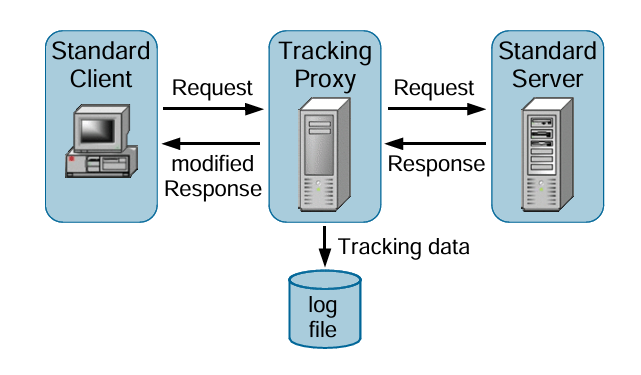
\includegraphics[width=0.5\textwidth]{2_Proxy_Server_Konzept}
\caption{HTTP-Proxy zur Ermittlung von Nutzerverhalten. Quelle: \cite{atterer2006knowing}}
\label{fig:proxy_server_concept}
\end{figure}

Der Proxy hat die Aufgabe, den HTTP-Content bzw. die HTML-Seite so zu bearbeiten, dass beispielsweise mittels JavaScript Verhaltensdaten im Client gesammelt und an den Proxy übermittelt werden. Die Bearbeitung des HTML erfolgt durch das Injizieren eines Skript-Tags in die Datei. Diese Daten werden anschließend vom Proxy in ein Logfile geschrieben, das zur Auswertung des Nutzerverhaltens dient. Eine Anpassung des Tracking-Codes erfordert somit keine Änderung des Produktivcodes, wodurch Flexibilität gewonnen wird. Wie im Abschnitt \ref{sec:solutions_tracking} erläutert, bleiben der Tracking-Code und die eigentliche Anwendungslogik voneinander getrennt. Dies hat zur Folge, dass der Code wartbar und verständlich bleibt.

\subsubsection{Funktionsweise des injizierten Skripts}
Das injizierte JavaScript bietet im Client die Möglichkeit, mittels DOM Events \cite{mdn2025_domevents} Mausbewegungen und Tastatureingaben und damit die Interaktion mit der Webseite zu erfassen. Die Registrierung auf Events hat dabei keine Auswirkungen auf den bestehenden JavaScript-Code, sofern keine Fehler im injizierten Skript vorhanden sind.

\subsubsection{Weitere Informationsgewinnung}
Unabhängig vom injizierten JavaScript-Code kann der Proxy auch die für einen Serverlog typischen Informationen (z.B. IP-Adresse, Gerätetyp usw.) erfassen. Da der Proxy zwischen Server und Client liegt, erscheint es für den Anwender so, als würde dieser direkt mit dem Server interagieren.

\subsubsection{Anwendbarkeit des Proxy-Ansatzes}
Das Proxy-System funktioniert aufgrund des Abhörens des gesamten HTTP-Verkehrs und des Einfügens von JavaScript sowohl für Single-Page- als auch für klassische Multi-Page-Applikationen.

\subsection{Externes JavaScript}
\label{subsec:external_js}
Ähnlich wie bei der in Unterabschnitt \ref{subsec:proxy_server} beschriebenen Proxy-Variante wird auch hier JavaScript eingesetzt. Im Gegensatz dazu erfolgt die Kommunikation jedoch nicht über einen Proxy, sondern über einen externen Server (siehe Abbildung \ref{fig:external_javascript}), wie dies beispielsweise bei Google Analytics \cite{weber2015practical} der Fall ist. Das Skript-Tag wird dabei direkt in jede Seite eingebettet, und das Skript wird vom Client vom Tracking-Server heruntergeladen. Anschließend sendet der Client die erfassten Daten über einen HTTP-Request direkt an den Tracking-Server.  
Die Informationen, die in der Proxy-Variante (Unterabschnitt \ref{subsec:proxy_server}) durch den Proxy ermittelt werden, können nun vom Browser selbst über asynchrone HTTP-Anfragen übertragen werden.

\begin{figure}[H]
\centering
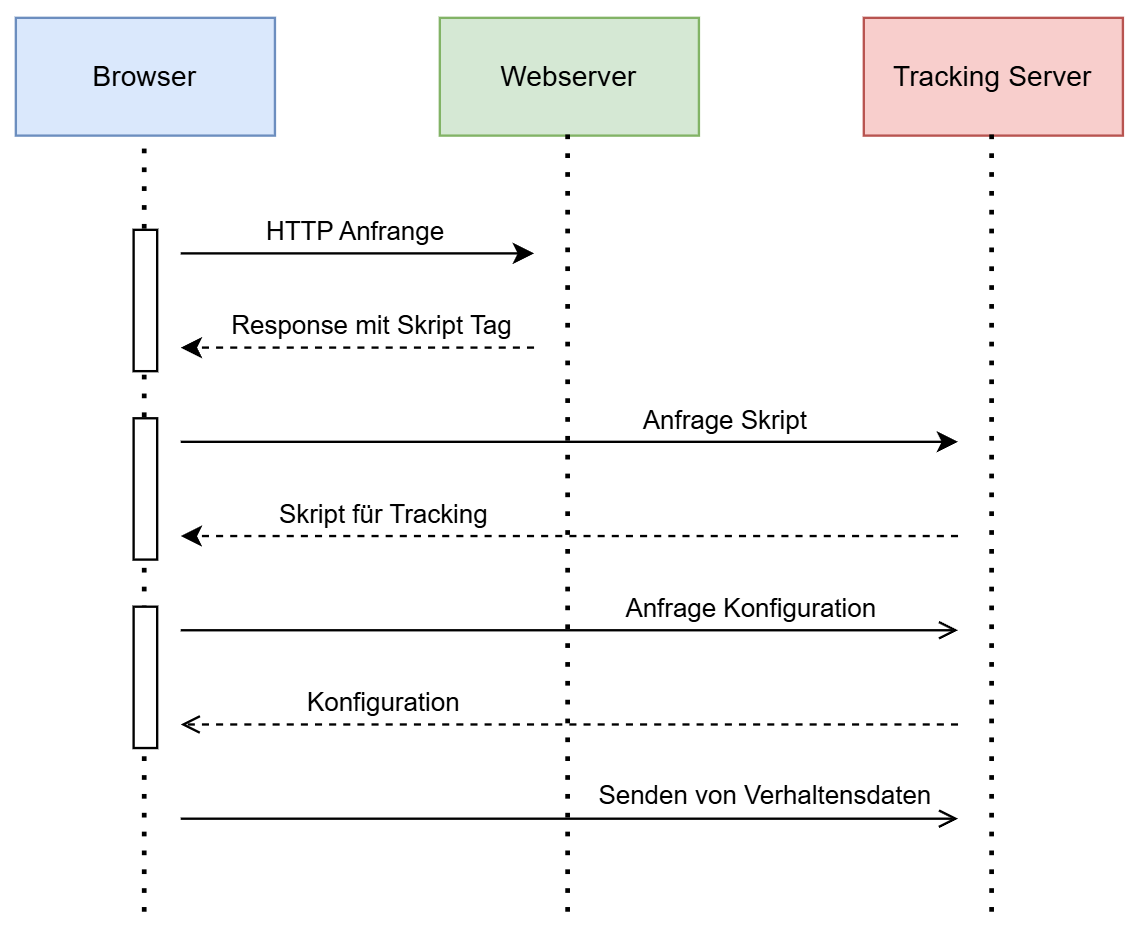
\includegraphics[width=0.6\textwidth]{2_Externes_Javascript}
\caption{Ablauf einer Standardinteraktion beim Tracking mit externem Skript.}
\label{fig:external_javascript}
\end{figure}

\subsubsection{Konfigurierbarkeit}
Die zu erfassenden Daten können von einem Konfigurationsserver, wie in Abbildung \ref{fig:external_javascript} veranschaulicht, abgefragt werden. Je nach übermittelter Konfiguration verhält sich das eingebundene Skript unterschiedlich, sodass die zu sammelnden Daten in Echtzeit und in gewünschter Form angepasst werden können. In Google Analytics (Unterabschnitt \ref{subsec:google_analytics}) wird diese Flexibilität beispielsweise durch den Tag Manager ermöglicht.

\subsubsection{Trennung von Aufgabenbereichen}
Da das Skript nun fest im Anwendungscode referenziert wird, kann es zusätzlich für benutzerdefinierte Aktionen innerhalb der Anwendung verwendet werden. Dadurch lassen sich sehr spezifische, auf den jeweiligen Anwendungsfall zugeschnittene Abfragen umsetzen. Grundsätzlich bleibt dabei eine Trennung zwischen Anwendungscode und Tracking-Code bestehen, solange kein benutzerdefiniertes Tracking implementiert wird.  
Das in Unterabschnitt \ref{subsec:proxy_server} beschriebene Proxy-Server-Konzept gilt hingegen als weniger transparent für Entwicklerinnen und Entwickler, während die feste Referenzierung des externen Scripts hier klare Anhaltspunkte für Verwendung und Zugriff bietet.

\subsection{Automatisch generierter Code}
\label{subsec:autogenerated_code}
Bereits im Unterabschnitt \ref{subsec:open_telemetry} wurde über eine Art von automatischem Tracking für die automatische Manipulation von Code gesprochen. Dadurch wird erreicht, dass der bestehende Code nicht angepasst werden muss und basierend auf Merkmalen im Produktivcode an bestimmten Stellen vordefinierter Code eingefügt wird (bei PostSharp z.B. Attribute). Dies kann je nach Technologie zur Laufzeit (z.B. mit der CLR Profiling API \cite{microsoft2025profiling}) oder zur Kompilierzeit (z.B. mit PostSharp \cite{postsharp-how-it-works}) geschehen.

\subsubsection{Beispiel OpenTelemetry und .NET}
OpenTelemetry realisiert das automatische Tracking für .NET (Abschnitt \ref{sec:dotnet}) über die CLR Profiling API \cite{microsoft2025profiling}. In Abbildung \ref{fig:opentelemetry_design} wird veranschaulicht, wie OpenTelemetry einen Profiler bereitstellt, der entsprechenden Code aus dem OTel SDK zur Laufzeit in den IL-Bytecode einfügt und Metainformationen für den geänderten Code bereitstellt. Der Profiler empfängt bestimmte Events, wie z.~B. das Event, dass eine Methode vom Just-in-Time (JIT) Compiler übersetzt wird. Daraufhin kann diese Methode angefordert und modifiziert werden. Die von der Common Language Runtime (CLR) bereitgestellte API erfordert jedoch umfangreiches Wissen über die CLR sowie den Aufbau von Assemblies \cite{Mikunov2003}.

\begin{figure}[H]
\centering
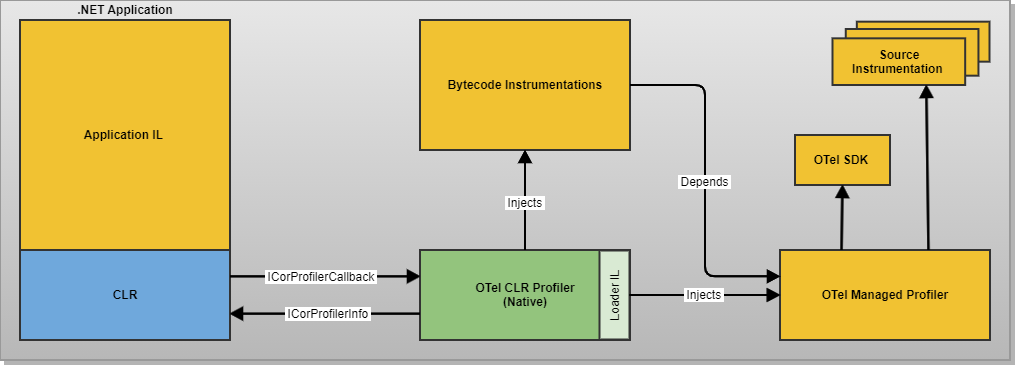
\includegraphics[width=0.9\textwidth]{2_OpenTelemetry_Auto_Mode_Design}
\caption{Aufbau des automatischen Telemetrierens unter .NET und OpenTelemetry. Quelle: \cite{otel-dotnet-instrumentation-design}}
\label{fig:opentelemetry_design}
\end{figure}

\subsubsection{Transparenz und Schwierigkeitsgrad}
Der im Hintergrund laufende Code, der mit der Anwendung agiert, kann grundsätzlich bestehenden Code verändern und nicht nur neuen hinzufügen. Daher besteht die Gefahr, dass bestimmtes Verhalten nicht mehr nachvollziehbar ist, insbesondere für Entwickler, die die ursprüngliche Anwendung entwickelt haben. Des Weiteren wird, wie in einem Artikel \cite{Mikunov2003} im MSDN erläutert, deutlich, dass es sich um ein komplexes Thema handelt. Die Implementierung mit C\# (Unterabschnitt \ref{subsec:csharp}) kann problematisch sein, da der .NET-Code erst vom JIT-Compiler übersetzt wird und auch Callbacks auslöst, die sorgfältig verarbeitet bzw. gefiltert werden müssen.

\subsection{Aufgabendelegation}
\label{subsec:task_delegation}
In Unterabschnitt \ref{subsec:autogenerated_code} und Unterabschnitt \ref{subsec:proxy_server} wurden bereits Konzepte vorgestellt, die in der Regel ein gesamtes System erfordern, dafür aber eine klare Trennung zwischen Anwendungscode und Tracking-Code ermöglichen.  
Es gibt jedoch weitere Ansätze, die Cross-Cutting Concerns \cite{crosscutting} berücksichtigen, ohne sie innerhalb einer einzelnen Klasse oder Methode zu vermischen.  
Eines dieser Konzepte ist die Delegation, die sich durch verschiedene Designansätze wie das Event-Driven Design (siehe Unterabschnitt \ref{subsubsec:event_driven_design}) und das Decorator Pattern umsetzen lässt.

\subsubsection{Event-Driven Design}
Event-Driven Design ist ein grundlegendes Konzept, bei dem Aktionen als Reaktion auf das Eintreten bestimmter Ereignisse ausgeführt werden.  
Die Komponenten, die auf ein Ereignis reagieren, sind dabei voneinander unabhängig.  
Handler registrieren sich für ein Event, sodass der Auslöser lediglich den Event-Endpunkt kennen muss.  
Dies führt zu einer losen Kopplung zwischen den beteiligten Komponenten, wobei lediglich eine gemeinsame Schnittstelle definiert werden muss.  

Im Kontext des Trackings bedeutet dies, dass sich der Tracking-Code bei einem Objekt registriert und benachrichtigt wird, sobald ein relevantes Ereignis auftritt. Der bestehende Anwendungscode muss den Tracking-Code also nicht direkt kennen. Das Event-Driven Design kann beispielsweise mithilfe des Observer Patterns der Gang of Four (GoF) \cite{gamma1995design} umgesetzt werden.

\subsubsection{Decorator Pattern}
Das Decorator Pattern der Gang of Four (GoF) \cite{gamma1995design} ermöglicht es, bestehendem Code zusätzliche Funktionalität hinzuzufügen, ohne diesen direkt zu verändern.  
Dabei hält eine neue Klasse eine Instanz einer bestehenden Klasse und erweitert deren Verhalten (siehe Abbildung \ref{fig:decorator_pattern}). 
Die Schnittstelle der dekorierten Klasse bleibt dabei identisch, und nach Ausführung der zusätzlichen Funktionalität werden die Aufrufe an die untergeordnete Instanz weitergeleitet. Dies ermöglicht eine saubere Trennung der Verantwortlichkeiten. Voraussetzung ist jedoch, dass das bestehende System bereits auf Interfaces basiert, da der Austausch von Komponenten andernfalls tiefgreifende Eingriffe in die Anwendung erfordern würde.

\begin{figure}[H]
\centering
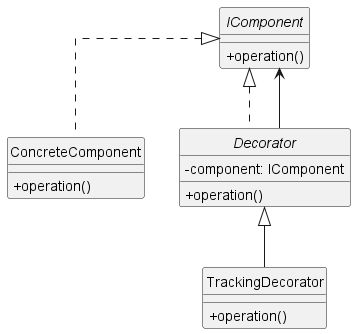
\includegraphics[width=0.5\textwidth]{2_Decorator_Pattern}
\caption{Decorator Pattern Klassendiagramm}
\label{fig:decorator_pattern}
\end{figure}

\section{Softwaremuster für UI-Frameworks}
\label{subsec:patterns}

Das im Zuge dieser Arbeit entwickelte Tracking-Framework soll in eine Windows Forms- (Unterabschnitt \ref{subsec:Winforms}) und eine WPF-Anwendung (Unterabschnitt \ref{subsec:WPF}) integriert werden. 
Für die Integration ist es daher wichtig zu verstehen, wie diese Anwendungen grundsätzlich aufgebaut sind. 
In diesem Abschnitt werden daher die Patterns MVVM (Unterabschnitt \ref{subsec:mvvm}) und MVP (Unterabschnitt \ref{subsec:mvp}) erläutert.

\subsection{MVVM}
\label{subsec:mvvm}

Das Model-View-ViewModel (MVVM) Pattern stammt von Microsoft \cite{Gossman2005MVVM} und wurde im Zuge der Entwicklung von WPF vorgestellt. 
Das Model-View-Controller (MVC) Pattern \cite{Krasner1988MVC} bildet dabei die Grundlage, wobei die Aufgabe des Models in beiden Patterns gleich bleibt. 
Der Zusammenhang zwischen den einzelnen Komponenten wird in Abbildung \ref{fig:mvvm_pattern} dargestellt.

\begin{figure}[H]
    \centering
    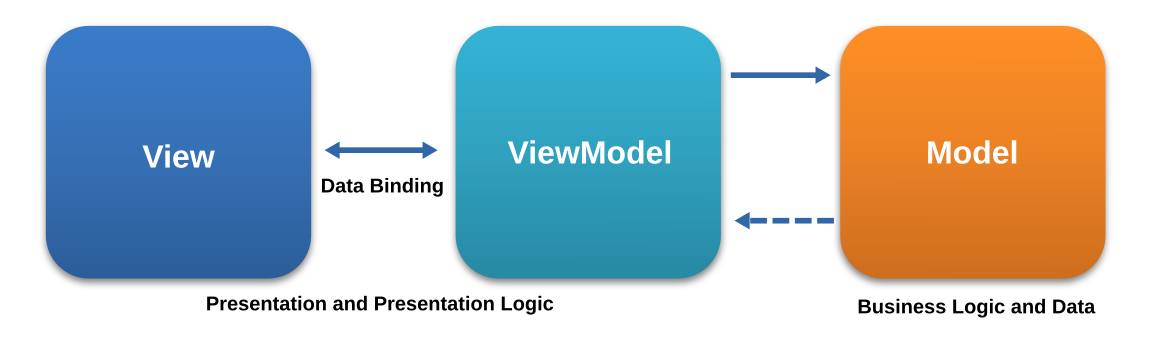
\includegraphics[width=0.7\textwidth]{2_MVVM_Pattern}
    \caption{Struktur des MVVM-Patterns. Quelle: \cite{Uncopy2024MVVMPattern}}
    \label{fig:mvvm_pattern}
\end{figure}

\subsubsection{View}
\label{subsubsec:view_for_mvvm}
Die View stellt gemeinsam mit dem ViewModel den Präsentations-Layer dar. Der Code für die View wird häufig durch sogenannte Designer \footnote{Programme, die eine Benutzeroberfläche bereitstellen, mit deren Hilfe UI-Elemente platziert und der Stil festgelegt werden kann. 
Diese Tools ermöglichen es Designern, auch ohne Programmierkenntnisse eine Benutzeroberfläche zu erstellen.} erzeugt und in einem XML-basierten Format wie z.\,B. XAML (in WPF) gespeichert. Die View enthält ausschließlich visuelle Elemente sowie die Logik, die für die Anzeige erforderlich ist (z.\,B. Animationen). Views, die Daten anzeigen, werden, wie in Abbildung \ref{fig:mvvm_pattern} gezeigt, über ein DataBinding mit den benötigten Informationen versorgt. Dazu hält die View eine Referenz auf das ViewModel, um das Binding herzustellen.

\subsubsection{Model}
\label{subsubsec:model_for_mvvm}
Die Business-Logik bzw. Domain-Logik enthält das Datenmodell, das unabhängig von der View und dem ViewModel verwendet werden kann. 
Daher besteht eine strikte Trennung zwischen Präsentationsschicht und Model. 
Dies ermöglicht die Wiederverwendung des Models in verschiedenen Anwendungen, ohne dass Änderungen an der Darstellung Anpassungen im Model erfordern. 
Zum Model zählen in der Regel Service-Methoden, Repositories und Entitäten. 
Das ViewModel bezieht, wie in Abbildung \ref{fig:mvvm_pattern} dargestellt, seine Daten aus diesem Model.

\subsubsection{ViewModel}
Das ViewModel fungiert als Adapter zwischen View und Model. In einfachen Fällen könnte die View direkt an das Model binden, was jedoch in komplexeren Szenarien dazu führen würde, dass das Model an die View angepasst werden müsste. Das ViewModel bereitet die Daten so auf, dass sie über das DataBinding der View bereitgestellt werden können. 
Ein weiterer Grund für die Einführung des ViewModels liegt darin, die für das Binding notwendige Logik aus der Domain-Logik herauszulösen, um diese sauber zu halten.

\subsubsection{DataBinding}
Das DataBinding (siehe Abbildung \ref{fig:mvvm_pattern}) ist der Datenkanal, über den Informationen zwischen zwei Komponenten in beide Richtungen ausgetauscht werden können. 
Beide Seiten werden über Datenänderungen informiert und synchronisieren sich je nach Art des Bindings automatisch.

\subsection{MVP}
Wie bereits das in Unterabschnitt \ref{subsec:mvvm} beschriebene Model–View–ViewModel (MVVM) Pattern hat auch das Model–View–Presenter (MVP) Pattern seinen Ursprung im Model–View–Controller (MVC) Pattern \cite{Krasner1988MVC}. 
IBM entwickelte daraus die erste Version dieses Patterns, wie im Artikel \cite{potel1996mvp} beschrieben wird. 
Die für diese Arbeit relevante Variante, das sogenannte \textit{Passive View Pattern}, wird in einer Publikation zu den sogenannten MV*-Patterns \cite{mvp_ieee} erläutert und bildet die Grundlage für einen Teil dieser Arbeit.

\begin{figure}[H]
    \centering
    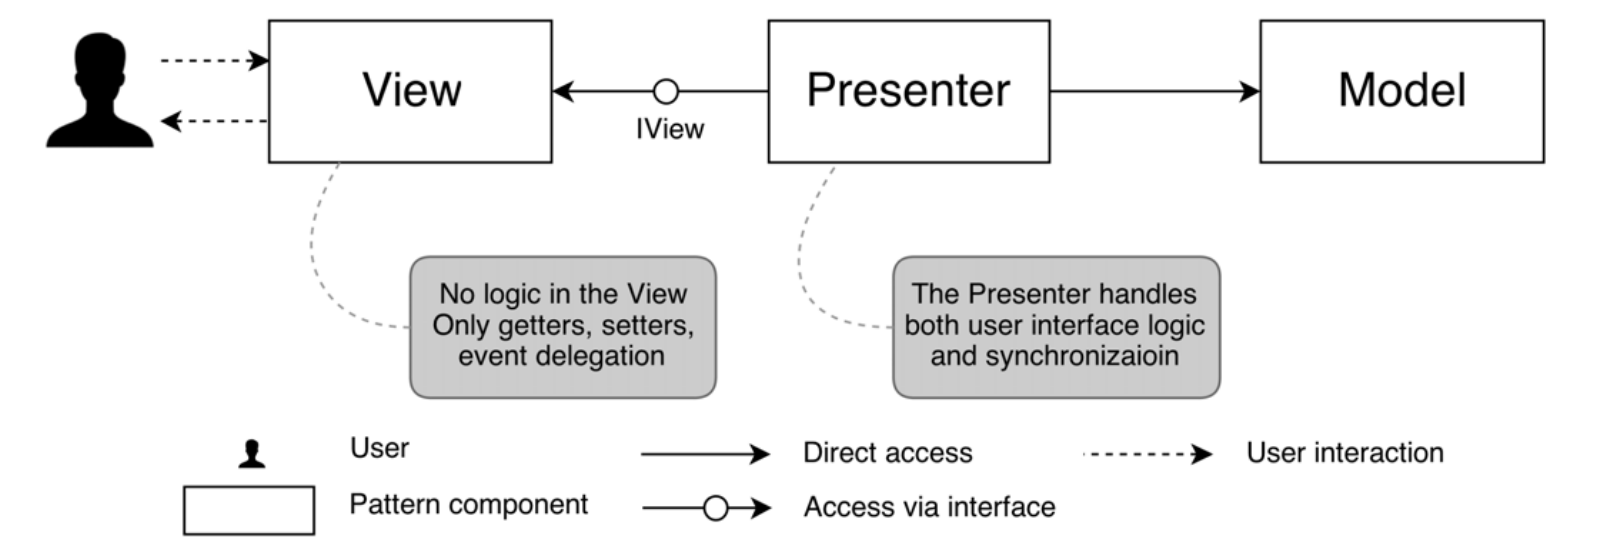
\includegraphics[width=0.8\textwidth]{2_MVP_Passive_View_Pattern}
    \caption{Passive View MVP Pattern. Quelle: \cite{mvp_ieee}}
    \label{fig:mvp_pattern}
\end{figure}

\subsubsection{Struktur des MVP-Patterns}
Das MVP-Pattern besteht aus einer View, einem Presenter und einem Model, wie in Abbildung \ref{fig:mvp_pattern} dargestellt. Das Model enthält, wie bereits beim MVVM-Pattern (Unterabschnitt \ref{subsec:mvvm}) erwähnt, die Domain-Logik und ist unabhängig von View und Presenter. 
Die View besteht ausschließlich aus Code, der für die Darstellung der Benutzeroberfläche notwendig ist, und enthält keinerlei Logik. Der Presenter übernimmt daher die gesamte Präsentationslogik und die Beschaffung der benötigten Daten aus dem Model. Der Presenter hält Referenzen sowohl auf die View als auch auf das Model. Die View wiederum informiert den Presenter über Benutzerinteraktionen, typischerweise über Events, wodurch keine Kopplung von der View zum Presenter entsteht. Der Presenter reagiert auf diese Ereignisse, führt die entsprechende Anwendungslogik aus und synchronisiert die View mit den aktuellen Daten. Er übernimmt somit im Wesentlichen die Aufgaben, die im MVVM-Pattern durch das ViewModel und das DataBinding realisiert werden.











